% The manuscript for P1EDA, short paper.
%
\documentclass[11pt,letterpaper]{article}
\usepackage{authblk}
\usepackage{times}
\usepackage{latexsym}
\usepackage{microtype}
\usepackage{amsmath,amssymb}
%\usepackage{microtype}
\usepackage{graphicx}
\usepackage{url}
\usepackage{rotating}
\usepackage{naaclhlt2015}
\setlength\titlebox{6.5cm}    % Expanding the titlebox

%\title{Multi-Level Alignments for Extensible Multilingual Textual Entailment}
% SP NEW TITLE
%\title{Multi-Level Alignments As An Extensible Multilingual Basis \\ for
%  Textual Entailment Algorithms}
% GIL, slightly modified title.
% ``representation basis'', ``representation layer'' emphasis. 
\title{Multi-Level Alignments As An Extensible Representation Basis \\
  for Textual Entailment Algorithms}

% authors
% Gil, Sebastian, Vered, Ido, Vivi, Kathrin, Lili, Meni 

\author[1]{Tae-Gil Noh}
\author[2]{Sebastian Pad{\'o}}
\author[3]{Vered Shwartz}
\author[3]{Ido Dagan}
\author[4]{\authorcr Vivi Nastase} % Vivi explicitly wanted her name as this 
\author[5]{Kathrin Eichler}
\author[3]{Lili Kotlerman}
\author[3]{Meni Adler} 
\affil[1]{Department of Computational Linguistics, Heidelberg University, Germany}
\affil[2]{Institute for Natural Language Processing, Stuttgart University, Germany}
\affil[3]{Department of Computer Science, Bar Ilan University, Israel}
\affil[4]{Human Language Technology, Fondazione Bruno Kessler, Italy}
\affil[5]{Language Technology Lab, DFKI GmbH, Germany}

% e-mails (eh....) 
% Gil          noh@cl.uni-heidelberg.de
% Sebastian    pado@ims.uni-stuttgart.de
% Vered        vered1986@gmail.com 
% Ido          ido.k.dagan@gmail.com    (or dagan@cs.biu.ac.il) 
% Vivi         nastase@fbk.eu
% Kathrin      kathrin.eichler@dfki.de
% Lili         lili.dav@gmail.com
% Meni         meni.adler@gmail.com

\date{}

\begin{document}
\maketitle
\begin{abstract}
  % 
  % SP OLD TEXT
  %Textual Entailment (TE) technology has become more robust over the last
  %years. Nevertheless, state-of-the-art models still rely on
  %incompatible data representations, which makes exchange of
  %components very difficult in practice. 
  A major problem in research on Textual Entailment (TE) is the high
  implementation effort for TE systems. Recently, interoperable
  standards for annotation and preprocessing have been proposed. In
  contrast, the algorithmic level remains unstandardized, which
  makes component re-use in this area very difficult in
  practice.
%
%
% SP OLD TEXT
%  In this paper, we introduce {\em multi-level alignments} as a
%  general representation to store information relevant for recognizing
%  entailment that 
%
  In this paper, we introduce {\em multi-level alignments} as a
  central, powerful representation for TE algorithms that encourages
  modular, reusable, multilingual algorithm development.
  % that can store many kinds of information. 
  %, can be translated easily into features,
  %  and is applicable across languages. 
  We demonstrate that a pilot open-source implementation of
  multi-level alignment with minimal features competes with
  state-of-the-art open-source TE engines in three languages.
\end{abstract}

\section{Introduction}
A key challenge of Natural Language Processing is to determine what
conclusions can be drawn from a natural language text, a task known as
\textit{Textual Entailment} (TE, Dagan and Glickman
2004).\nocite{dagan04:_probab_textual_entail} The ability to recognize
TE helps dealing with surface variability in tasks like Question
Answering~\cite{harabagiu-hickl:2006:COLACL}, Intelligent Tutoring
\cite{nielsen09:_recog_entail_in_intel_tutor_system}, or Text
Exploration \cite{berant2012learning}. Open source implementations a
number of TE algorithms have become available over the last years,
including BIUTEE \cite{Stern:2012} and EDITS \cite{Kouylekov:2010},
which has made it much easier for end users to utilize TE engines.

At the same time, the situation is still more difficult for
researchers and developers. Even though recently a common platform for
TE has been proposed \cite{EOP-arch} that standardizes important
aspects like annotation types, preprocessing, and knowledge resources,
it largely ignores the algorithmic level. In fact, TE algorithms
themselves are generally not designed to be extensible or
interoperable. Therefore, changes to the algorithms -- like adding
support for a new language or for new analysis aspect -- are often
very involved, if not impossible. This often forces the next
generation of TE researchers to develop and implement their own core
algorithms from scratch.

%TE technology has matured substantially over the last decade. Numerous
%engines have been developed that implement a wide range of algorithms
%and make use of many types of linguistic knowledge resources.

%However, developers and researchers are still out of luck: 
%However, 

In this paper, we address this problem by proposing a schema for TE
algorithms that revolves around a central representation layer called
{\em multi-level alignment} geared towards encoding the relevant
information for deciding entailment. The use of multi-level
alignments encourages a modular, extensible development of TE
algorithms that can be partitioned into ``alignment producers'' and
``alignment consumers''. This enables for future researchers
and developers to change analysis components or add new ones in a
straightforward manner.
%\marginpar{SP: that's just a claim, right?}
%Gil: I agree. ``producer'' ``consumer'' sounds also clear. 

We also present evaluation results for a very simple TE algorithm
based on multi-level alignments for English, German and Italian. It
utilizes a minimal set of analyzers and four basic
language-independent features. It can thus be regarded as a baseline
of the performance achievable with this approach.  The results can
already compete with the best open-source engines available for each
of the languages.

\section{TE with Multi-Level Alignments}

The quality of the word alignment between a Text (T) and a Hypothesis
(H) has been used very early as a simple feature to decide about
TE. When it was found that alignment strength  can be
misleading \cite{maccartney-EtAl:2006:HLT-NAACL06-Main}, alignment was
understood as an intermediate step whose outcome is a set of
correspondences between parts of T and H that can be used to define
(mis-)match features. Alignments can be established at the word level,
phrase level \cite{MacCartney:EMNLP08}, or dependency level
\cite{dinu-wang:2009:EACL}. Dagan et al. \shortcite{RTE-book}
generalized this practical use to an architectural principle: They
showed that various TE algorithms can be mapped onto a universal
alignment-based schema with six steps: pre-processing, enrichment,
candidate alignment generation, alignment selection, and
classification.

\paragraph{Proposal.} Our proposal is similar to, but simpler than,
Dagan et al.'s. Figure \ref{fig:1} shows the data flow.

\begin{figure}[t!b]
  \centering
  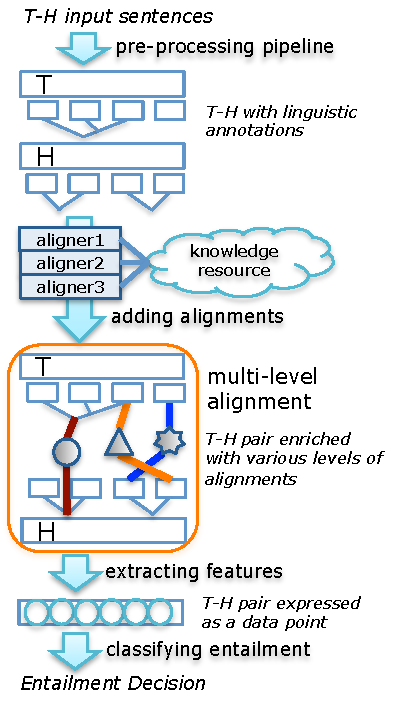
\includegraphics[width=0.9\columnwidth]{figures/figure1.pdf}
  \caption{Dataflow for TE algorithms based on multi level alignment}
  \label{fig:1}
\end{figure}

First, the text and the hypothesis are linguistically
pre-processed. Then, the annotated T-H pair becomes the input for
various independent aligners, which have access to knowledge resources
and can compute any evidence for or against entailment that can be
represented as a weighted alignment between any linguistic levels of H
and T.
Note that this includes many analyses not normally treated as
alignment, e.g. match or mismatch in negation or modality between
parts of T and H. %, or the location of inference rules.
The union of all alignments forms the 
central data structure, the {\em Multi-Level Alignments}.

The next step is feature extraction. Features can be extracted on the
basis of individual alignments, or from sets of alignments. We assume
that the features form a vector describing the T-H pair, and that the
last step is supervised entailment classification.

\paragraph{Discussion.} The main difference to Dagan et al.'s schema
is that we intentionally leave out the step of {\em alignment
  selection} which explicitly selects a single alignment for each part
of H or T, typically the globally most probable one.  Our decision to
forgo selection is grounded in our design of multi-level alignments as
a repository that supports coexistence of information from different
sources. This has the following benefits: (a) aligners become
decoupled in that adding a new aligner does not have a direct impact
on other aligners;
%in that adding a new aligner does not have a direct impact
%on the global outcome;
(b) alignments produced by different aligners
can have different semantics, e.g. positive (match) or negative
(mismatch); (c) interactions between alignments can still be captured
by defining features in the feature extraction step.

In this manner, multi-level alignments serve as an abstraction layer
that encourages the development of TE algorithms composed of small,
self-contained modules that solve specialized tasks in TE
recognition. Each of these modules consists of two parts: an aligner,
and a set of feature extractors. A priori, each module can be defined
independently; to introduce interactions with other modules, it should
be sufficient to extend the feature extractors.

The practical benefit for the developer is that even relatively
complex TE algorithms use a small set of well-defined interfaces,
which makes them easy to manage, even at the implementation level. The
startup cost is getting acquainted with the common data structure of
multi-level alignments. We believe that developers are willing to pay
this cost, especially when this provides them with a platform that
supports multilingual pre-processing and resources. 

\section{Implementation and Evaluation}
\label{sec:impl}

We describe an implementation of a pilot TE algorithm based on the
Multi-Level Alignment approach and its evaluation in three languages
(EN, DE, IT). The system is available as
open-source.\footnote{As a part of Excitement Open Platform for Textual Entailment. \url{https://github.com/hltfbk/EOP-1.2.1/wiki/AlignmentEDAP1}} 

%Multi-Level Alignment
%approach to test its potential by evaluating it on two use cases in
%three languages (DE, EN, IT). 

\subsection{Technical Foundations}  
\label{sec:techn-found}

We implement the algorithm within an open source TE development
platform \cite{EOP-arch}. The platform provides various multilingual
pre-processing pipelines and knowledge resources such as WordNet,
VerbOcean, etc., under a shared API. For pre-processing, we use
TreeTagger-based pipelines for all three languages.

Another important service provided by the platform is the
ability of storing a wide range of linguistic annotations in a common,
language-independent data representation. The platform uses UIMA CAS
\cite{d04:_uima} as the data container, adopts the DKPro type system
\cite{DKpro}, and defines annotation types which can be extended in a
controlled manner. We used this capability to define a multilingual
Multi-Level Alignment layer  %(links with types, labels and weights)
with little implementation effort.
%By
%utilizing those existing modules of a common platform, we were able to
%concentrate on the core-algorithm implementations.

\subsection{A Minimal Set of Aligners}

The pilot algorithm restricts itself to three aligners.  All three are
fully language-independent, even if two use
language-specific knowledge resources.

\paragraph{Lexical Aligner.} The lexical aligner adds an alignment link
for a pair of lemmas in T and H if it finds some kind of semantic
relationships between them in a set of lexical resources. The link is
directed, labeled (by the semantic relation, e.g. ``synonym'',
``antonym'') and weighted, with the weight indicating the strength of
the relationship. Note that this aligner can on its own already
produce alignment links with inconsistent semantics (positive and
negative). For English, WordNet and VerbOcean were used as lexical
resources. Italian WordNet was used for Italian, and GermaNet and
German DerivBase \cite{Zeller:2013} were used as lexical resources for
German.

\paragraph{Paraphrase Aligner.} The paraphrase aligner concentrates on
surface forms rather than lemmas and can align sequences of them
rather than just individual tokens. It uses paraphrase tables, e.g.
extracted from parallel corpora
\cite{bannard05:_parap_bilin_paral_corpor}. The alignment process is
similar to the lexical aligner: any two sequences of tokens in T and H 
are aligned if the pair is listed in the resource.  The alignment
links created by this aligner instantiate only one relation
(``paraphrase'') but report the strength of the relation via the
translation probability. We used the paraphrase tables provided by the
METEOR MT evaluation package \cite{denkowski-lavie:2014:W14-33}, which
are available for numerous languages. 

\paragraph{Lemma Identity Aligner.} This aligner does not use any
resources. It simply aligns identical lemmas between T and H and plays
an important role in practice to deal with named entities.

\subsection{A Minimal Feature Set} 

Similar to the aligners, we concentrate on a small set of four
features in the pilot algorithm. Again, the features are completely
language independent, even at the implementation level. This is
possible because the linguistic annotations and the alignments, use a
language-independent type system (cf. Section~\ref{sec:techn-found}).

All current features measure some form of \textit{coverage} on the
Hypothesis, i.e. the percentage of H that can be explained by T. The
underlying hypothesis is that a higher coverage of H corresponds to a
higher chance of entailment. Since parts-of-speech arguably differ in
the importance of being covered, we compute coverage for four sets of
words separately: (a), for all words; (b), for content words; (c), for
verbs; (d), for proper names (according to the POS tagger). The
features are defined on the union of all produced alignments: i.e.,
two words count as aligned if they were aligned by any aligner. 
Clearly, this is an overly simplistic (albeit surprisingly effective)
strategy. It can be considered a baseline for our approach that can be
extended with many features that suggest themselves from the
literature. 

\section{Experimental Evaluation} 
 
\paragraph{Evaluation 1: RTE-3.}
RTE-3 was the third instance of the yearly benchmarking workshops of
the Textual Entailment community
\cite{giampiccolo07:_third_pascal_recog_textual_entail_chall}. The
English dataset created for RTE-3 consists of 800 training and 800
testing T-H pairs. Later, the RTE-3 dataset was translated into both
German and Italian \cite{Magnini:2014}. %This makes
It is the only Textual Entailment dataset in multiple languages with
the same content. The task is binary TE recognition, with baseline of
50\% accuracy (balanced classes).

We trained and tested our Multi-Level Alignment approach ({\em
  MultiAlign}) on the RTE-3 dataset separately for each language. We
compare against the other RTE systems from the platform by Pad\'o et
al. \shortcite{EOP-arch}, namely BIUTEE \cite{Stern:2012}, EDITS
\cite{Kouylekov:2010}, and TIE \cite{Wang:2009}. Each system is
configured with its best known configurations. The pilot system
supports all three languages, while others support one (BIUTEE) or
two languages (EDITS, TIE).

\begin{table}[t!]
\centering
%\small
\begin{tabular}{l|ccc}
          &   English   &   German   &   Italian \\
\hline
{\em MultiAlign}&   \textbf{67.0}      &   \textbf{64.5}    &  \textbf{65.4}  \\
BIUTEE        &   \textbf{67.0}      &     -       &     -    \\
TIE           &   65.2       &   63.1    &     -    \\ 
EDITS         &   63.6      &     -       &  62.6  \\ \hline
RTE3 median   &   61.8      &             &          \\

\end{tabular}
\caption{Accuracy evaluation on the RTE3 dataset}
\label{table:rte3}
\end{table}

The results are shown in Table~\ref{table:rte3}. The pilot system
performs well in all three languages. It ties with BIUTEE on English
and it outperforms TIE and EDITS in their respective results on German
and Italian. This is particularly notable since all three systems have
gone through several years of development, while {\em MultiAlign} is
only a pilot implementation. 

%\paragraph{Evaluation 2: T-H pairs from Entailment Graphs}
\paragraph{Evaluation 2: T-H pairs from Application Data.}
We perform the second evaluation on real-world application data from
two application datasets: an entailment graph dataset (for English and
Italian), and an e-mail categorization dataset (for German).
%Entailment graphs are graphs whose nodes are sets of statements,
%and whose edges represent entailment relations.
Entailment graph building is the task of constructing graphs that
hierarchically structure the statements from a collection
\cite{berant2012learning} for the application of Text Exploration.  In
TE-based e-mail categorization, the goal is to assign the right
category to an email with TE, using the email as T and a category
description as H. \cite{Eichler:2014}.

Due to space constraints, we cannot evaluate these applications
end-to-end. Instead, we focus on the respective first step, the binary
decision of entailment for individual T-H pairs. This task corresponds
to RTE-3, and the main difference to Evaluation~1 is that these pairs
come from real-world interactions and were produced by native
speakers.  All T-H pairs %of the three languages
are sampled from application gold data which were manually constructed
on the basis of anonymized customer interactions (Eichler et
al. \shortcite{Eichler:2014} for German; Kotlerman et
al. \shortcite{Kotlerman:2015} for English and Italian\footnote{Both
  datasets are publicly available.}). The sets are fairly large (5300
pairs for English, 1700 for Italian, 1274 for German), and were
sampled to be balanced. We report F$_1$ for comparability with
non-balanced setups (our random baseline is F$_1$=50). 

%The second evaluation is on T-H pairs from entailment graph
%data.

%Entailment graphs are graphs whose nodes are sets of statements,
%and whose edges represent entailment relations. Entailment graphs can
%drive Text Exploration applications where a user wants to obtain a
%hierarchical structuring of the statements from a collection 
%\cite{berant2012learning}.

% Due to space constraints, we cannot evaluate the end-to-end task of
% entailment graph construction. Instead, we focus on the first step,
% the binary decision of entailment for individual T-H pairs, similar to
% RTE-3.
%The main difference to RTE-3 is however that these T-H pairs
%come from real-world application data in the three languages and were
%produced by native speakers.
%They were sampled from entailment graphs
%that were manually constructed on the basis of anonymized real-world
%customer interactions datasets (REF\footnote{Omitted for
%  anonymity. The dataset is publicly available.} for English and
%Italian; Eichler et al. \shortcite{Eichler:2014} for German).  The
%sets were sampled to be balanced. We report F$_1$ for comparability
%with non-balanced setups; the random baseline in our setup is
%F$_1$=50. They are fairly large (5300 pairs for English, 1700 pairs
%for Italian, 1274 pairs for German).

\begin{table}[t!]
\centering
%\small
\begin{tabular}{l|ccc}
              &   English         &   German        &  Italian  \\
\hline
{\em MultiAlign}&   69.2          &  \textbf{72.4}  &  \textbf{69.5}   \\
BIUTEE          &   \textbf{71.3} &     -           &     -            \\
TIE             &     67.3        &  \textbf{72.4}  &     -            \\ 
EDITS           &     66.6        &     -           &    65.6          \\

\end{tabular}
\caption{F$_1$ evaluation on application data}
% balanced, pure-split data.  
\label{table:egraph}
\end{table}

Table \ref{table:egraph} shows our evaluation results.
{\it MultiAlign} system beats EDITS for Italian (+4), and ties
with TIE for German. On English, BIUTEE still outperforms {\it
  MultiAlign} (-2). Thus, {\it MultiAlign} also performs acceptably 
on real-world data. 

In sum, we find that {\it MultiAlign} is already competitive with
state-of-the-art open-source TE engines on three languages.  
{\it MultiAlign} is not only much less complex, but it is also a single
system covering all three languages, without any language-specific
optimizations. We interpret this as a positive sign for the future of
the Multi-Level Alignment approach.


% (added for final copy)
\paragraph{Visualization.}

The platform also supports visualization of individual Text-Hypothesis
pairs, showing the alignments that were created by the system as well
as the features computed on the basis of the alignments. The
visualization was built on the basis of the BRAT
library.\footnote{\url{http://brat.nlplab.org/index.html}}

\begin{figure*}[t]
  \centering
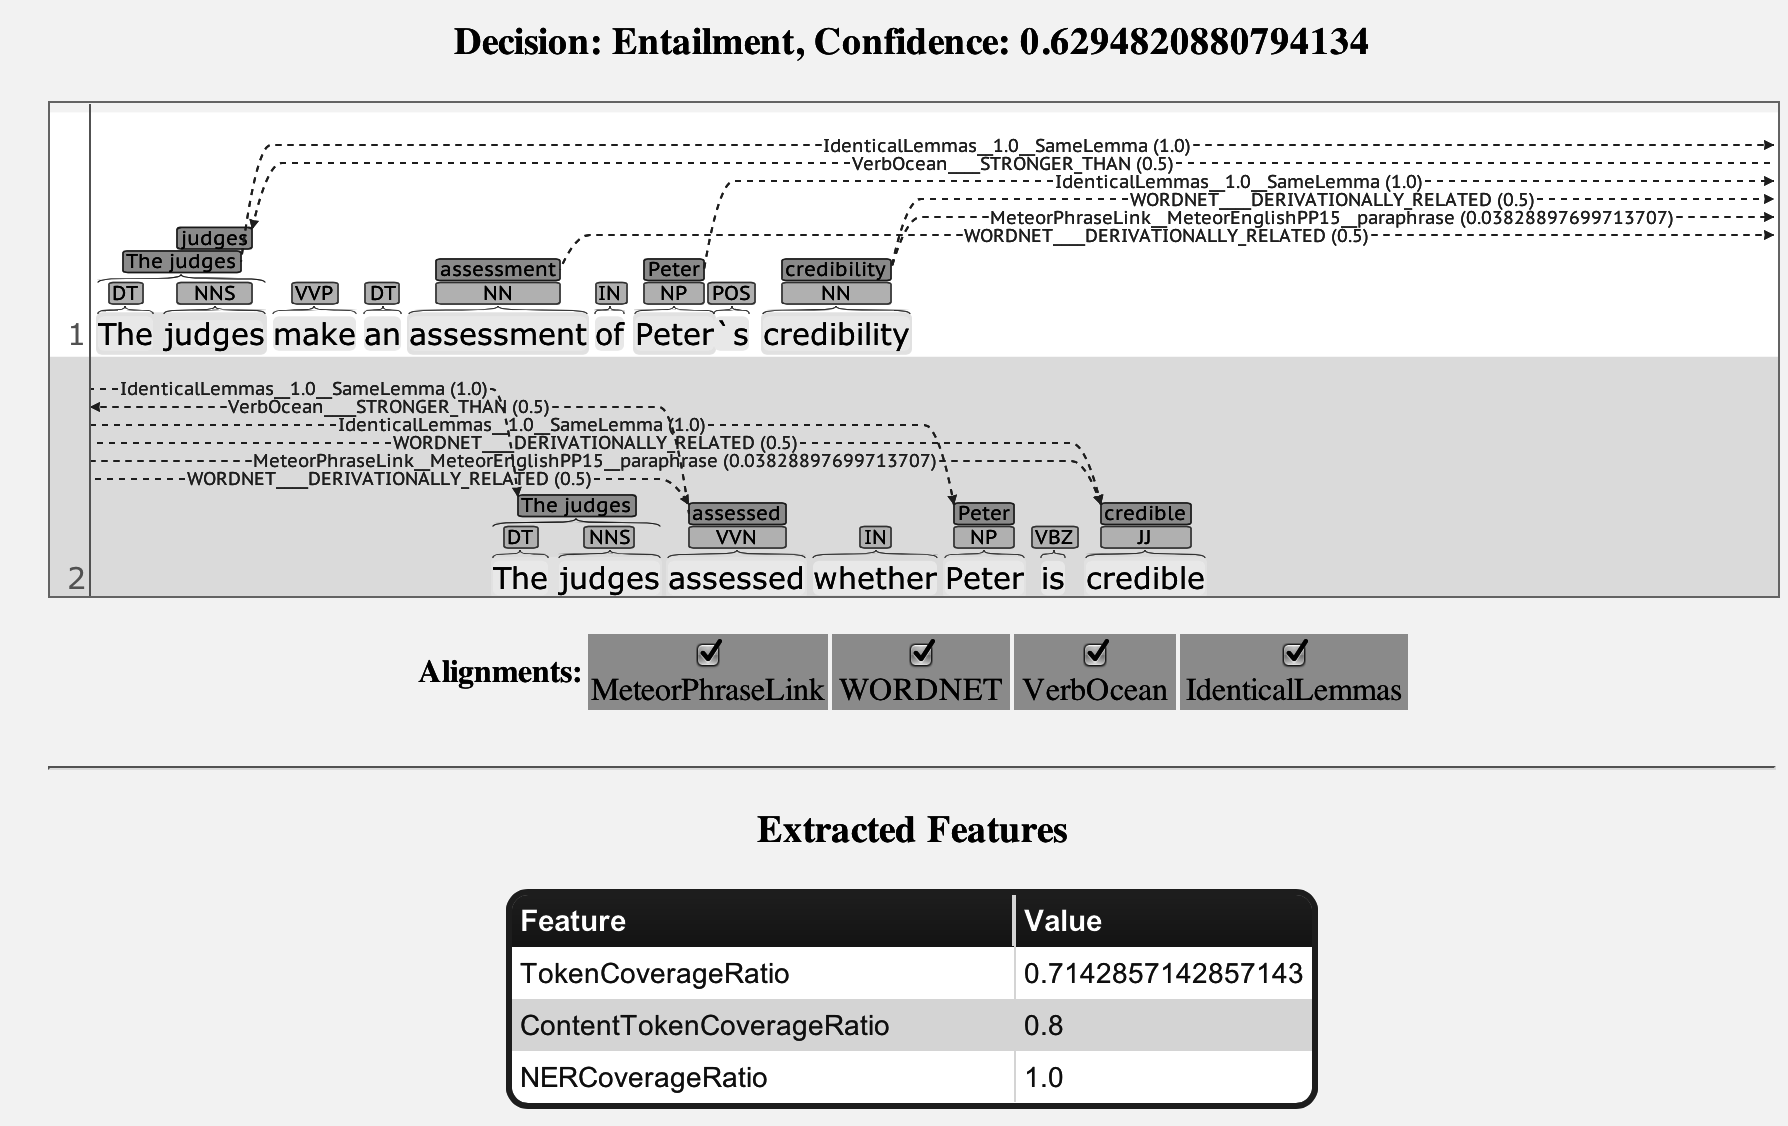
\includegraphics[width=\textwidth]{ScreenshotGray}  
  \caption{Screenshot of the Multi-Level Alignment Visualizer}
  \label{fig:screenshot}
\end{figure*}

Figure~\ref{fig:screenshot} shows an example for the Text \textit{The
  judges made an assessment of Peter's credibility} and the Hypothesis
\textit{The judges assessed if Peter was credible}. The top line shows
the final prediction, Entailment, and the confidence (75\%). The main
part shows the Text and the Hypothesis below each other, connected by
alignment links that are labeled with their source and their
score. Recall that we use WordNet and VerbOcean as knowledge sources
for the Lexical Aligner, Meteor for the Paraphrase Aligner, and
finally the Identical Lemma Aligner. Note that the alignments can link
individual words (\textit{assessment} and \textit{assess} are aligned
through a derivational link from WordNet) but also phrases (The two
occurrences of \textit{The judges} in Text and Hypothesis are linked
by virtue of being identical lemmas). 

The three features currently used by the English system are are shown
below. As can be seen, they aggregate very simple statistics about the
alignments: 5 of 7 tokens in the hypothesis are covered, 4 out of 5
content words, and the one proper name is also aligned. This situation
motivates nicely the use of those features: a relatively low alignment
coverage on all tokens is still compatible with entailment as long as
the crucial tokens are aligned. 

This visualization enables end users to quickly take in the
justification behind the system's decision. Developers can inspect
alignments and features for plausibility and detect possible bugs and
assess the limitations of aligners and their underlying resources. For
example, the current example shows a wrong link produced by the
VerbOcean resource between the noun \textit{judges} in the Text and
the verb \textit{assessed} in the Hypothesis. The reason is that the
noun \textit{judges} is mistaken for an inflected form of the verb
\textit{to judge} which indeed stands in a \textit{Stronger-than}
relationship to \textit{to assess}.

\section{Conclusion}

This paper proposed the use of {{\em multi-level alignments}, a rich
  data structure allowing multiple alignments to co-exist. We argued
  that multi-level alignments are a suitable basis for developing
  Textual Entailment algorithms by virtue of providing a beneficial
  abstraction layer that supports extensible and modular entailment
  algorithms. A pilot TE algorithm developed in this schema showed
  performance comparable to much more sophisticated state-of-the-art
  open-source TE engines and is available as open source software.
%The system is extensible, small and robust, and supports
%input in three languages. 
%It is available as open-source, and can be used by anyone who requires
%a multilingual TE engine.
%We believe that  can lead to more modular and more easily
%extensible TE engines.   

%% \section*{Acknowledgments}

%% Do not number the acknowledgment section.
\bibliographystyle{naaclhlt2015}
\bibliography{sem2015_short}

\end{document}
